\documentclass[10pt]{standalone}
\usepackage{stix}
\usepackage{tikz}
\usepackage{xcolor}
\usepackage{amsmath}
\usepackage{braket}
\usepackage{comment}
\definecolor{Fblue}{HTML}{560dcb}
\definecolor{Fred}{HTML}{92235a}
\definecolor{Firebrick}{HTML}{b22222}
\definecolor{Fnavy}{HTML}{000080}
\definecolor{ForangeRed}{HTML}{ff4500}
\definecolor{Fcornflower}{HTML}{bbddff}
\definecolor{Fcmix}{HTML}{0f4880}
\definecolor{Faqua}{HTML}{5fbf9f}
\definecolor{Fmagnifying}{HTML}{303030}
\newcommand{\bvec}[1]{\boldsymbol{#1}}
\usetikzlibrary{calc, arrows, arrows.meta, math} %, fpu}

\newcommand{\xp}[1]{\texttt{\color{ForangeRed}#1}}
\newcommand{\tp}[1]{\texttt{\color{Firebrick}#1}}
\newcommand{\tpd}[1]{\tp{#1} [displ,size]}
\newcommand{\ipd}[1]{#1 [displ, size]}

\newcommand{\bracketOne}[2]{
  \draw (cell#1.west) -- ++(-0.1,0.0) node {#2};
}
\newcommand{\bracketTwo}[3]{
  \tikzmath{\coordA = 0.5*(cell#1.west) + 0.5*(cell#2.west) + (-0.1,0.0);}
  \draw (cell#1.west) -- (\coordA);
  \draw (cell#2.west) -- (\coordA) node {#3};
}
\newcommand{\bracketThree}[4]{
  \tikzmath{\dbuf = 1./3.;
    \coordA = \dbuf*(cell#1.west) + \dbuf*(cell#2.west) + \dbuf*(cell#3.west) + (-0.1,0.0);}
  \draw (cell#1.west) -- (\coordA);
  \draw (cell#2.west) -- (\coordA);
  \draw (cell#3.west) -- (\coordA) node {#4};
}

\newcommand{\EbracketOne}[2]{
  \draw (Ecell#1.east) -- ++(0.1,0.0) node[anchor=west] {#2};
}
\newcommand{\EbracketTwo}[3]{
  \tikzmath{\coordA = 0.5*(Ecell#1.east) + 0.5*(Ecell#2.east) + (0.1,0.0);}
  \draw (Ecell#1.east) -- (\coordA);
  \draw (Ecell#2.east) -- (\coordA) node[anchor=west] {#3};
}
\newcommand{\EbracketThree}[4]{
  \tikzmath{\dbuf = 1./3.;
    \coordA = \dbuf*(Ecell#1.east) + \dbuf*(Ecell#2.east) + \dbuf*(Ecell#3.east) + (0.1,0.0);}
  \draw (Ecell#1.east) -- (\coordA);
  \draw (Ecell#2.east) -- (\coordA);
  \draw (Ecell#3.east) -- (\coordA) node[anchor=west] {#4};
}

\newcommand{\colorizeBox}[3]{
  \tikzmath{\coordA = (0,1-#1/64.0);
            \coordB = (1,1-#2/64.0);}
  \fill[draw=none, fill=#3] (\coordA) rectangle (\coordB);
}
\newcommand{\EcolorizeBox}[3]{
  \tikzmath{\coordA = (0,1-#1/64.0+67/64.0);
            \coordB = (1,1-#2/64.0+67/64.0);}
  \fill[draw=none, fill=#3] (\coordA) rectangle (\coordB);
}

\begin{document}
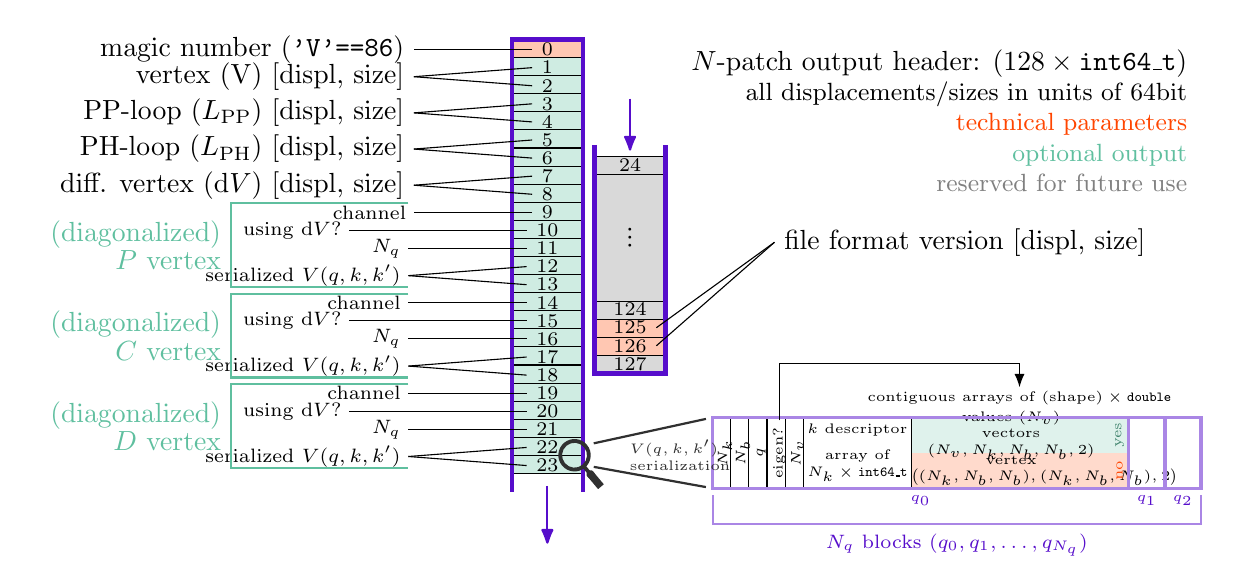
\begin{tikzpicture}[x=5.90552in, y=5.90552in, >={Latex[round]}]
  \clip (0,0.55) rectangle (1,1.0);
  \tikzmath{
    coordinate \coordA;
    coordinate \coordB;
    int \ibuf;
    real \dbuf;
  }
  \node[anchor=north east] at (0.99,0.99) {\begin{minipage}{3in}%
    \begin{flushright}%
      $N$-patch output header: $(128 \times \texttt{int64\_t})$\\
      \small
      all displacements/sizes in units of 64bit \\
      \textcolor{ForangeRed}{technical parameters} \\
      \textcolor{Faqua}{optional output} \\
      \textcolor{gray}{reserved for future use}
    \end{flushright}
  \end{minipage}};

  \begin{scope}[shift={(0.41,0.01)}, yscale=0.98, xscale=0.06]
    \colorizeBox{0}{1}{ForangeRed!30!white}
    \colorizeBox{1}{24}{Faqua!30!white}

    \foreach \idx in {1,2,...,24} {
      \tikzmath{
        \dbuf = 1./64.;
        \ibuf = \idx-1;
        \coordA = (0,1-\idx/64.0);
        \coordB = (1,1-\idx/64.0);
      }
      \draw (\coordA) -- node[midway, above, yshift=-0.29em] (cell\ibuf) {\scriptsize\ibuf} (\coordB);
    }
    \tikzmath{ \dbuf = 1. - 23./64. - 2./64.; }
    \draw[Fblue, ultra thick] (0,\dbuf) -- (0,1) -- (1,1) -- (1,\dbuf);
    \tikzmath{ \dbuf = \dbuf + 0.005; }
    \draw[Fblue, ->, thick] (0.5,\dbuf) -- ++(0,-0.05);
  \end{scope}
  \begin{scope}[shift={(0.48,-0.089)}, yscale=0.98, xscale=0.06]
    \EcolorizeBox{67}{76}{gray!30!white}
    \EcolorizeBox{78}{79}{gray!30!white}

    \EcolorizeBox{76}{78}{ForangeRed!30!white}

    \tikzmath{
      int \add;
      int \iloc;
      coordinate \ctmpOne;
      coordinate \ctmpTwo;
      for \idx in {0,1,...,4} {
        if \idx>0 then {
          \add = 123;
          \iloc = \idx + 7;
        } else {
          \add = 24;
          \iloc = \idx + 0;
        };
        \ibuf = \add + \idx;
        \coordA = (0,1-\iloc/64.0);
        \coordB = (1,1-\iloc/64.0);
        {
          \draw (\coordA) -- node[midway, below, yshift=0.27em] (Ecell\ibuf) {\scriptsize\ibuf} (\coordB);
        };
        if \idx==0 then {
          \coordA = (0,1-\iloc/64.0-1./64.);
          \coordB = (1,1-\iloc/64.0-1./64.);
          \ctmpOne = 0.5*(\coordA)+0.5*(\coordB);
          {
            \draw (\coordA) -- (\coordB);
          };
        } else { if \idx==1 then {
          \ctmpTwo = 0.5*(\coordA)+0.5*(\coordB);
        } else {}; };
      };
      \ctmpOne = 0.5*(\ctmpOne) + 0.5*(\ctmpTwo);
      {
        \node[anchor=center,rotate=90] at (\ctmpOne) {...};
      };
      \iloc = \iloc + 1;
    }
    \tikzmath{\dbuf = 1.0 - \iloc/64.0;}
    \draw[Fblue, ultra thick] (0,1.01) -- (0,\dbuf) -- (1,\dbuf) -- (1,1.01);
    \draw[Fblue, ->, thick] (0.5,1.05) -- (0.5,1.005);
  \end{scope}
  \begin{scope}[anchor=east]
    \bracketOne{0}{magic number (\texttt{'V'==86})}
    \bracketTwo{1}{2}{\ipd{vertex ($\mathrm{V}$)}}
    \bracketTwo{3}{4}{\ipd{PP-loop ($L_\mathrm{PP}$)}}
    \bracketTwo{5}{6}{\ipd{PH-loop ($L_\mathrm{PH}$)}}
    \bracketTwo{7}{8}{\ipd{diff. vertex ($\mathrm{d}V$)}}

    {\scriptsize
    \bracketOne{9}{channel}
    \draw (cell10.west) -- ++(-0.15,0.0) node {using $\mathrm{d}V$?};
    \bracketOne{11}{$N_q$}
    \bracketTwo{12}{13}{serialized $V(q,k,k')$}

    \bracketOne{14}{channel}
    \draw (cell15.west) -- ++(-0.15,0.0) node {using $\mathrm{d}V$?};
    \bracketOne{16}{$N_q$}
    \bracketTwo{17}{18}{serialized $V(q,k,k')$}

    \bracketOne{19}{channel}
    \draw (cell20.west) -- ++(-0.15,0.0) node {using $\mathrm{d}V$?};
    \bracketOne{21}{$N_q$}
    \bracketTwo{22}{23}{serialized $V(q,k,k')$}
    }

    \tikzmath{\coordA = 0.5*(Ecell125.east) + 0.5*(Ecell126.east) + (0.1,0.08);}
    \draw (Ecell125.east) -- (\coordA);
    \draw (Ecell126.east) -- (\coordA) node[anchor=west] {\ipd{file format version}};

    \tikzmath{\coordA = (cell10.west) + (-0.1,0.023);
              \coordB = (cell13.west) + (-0.1,-0.002);}
    \tikzmath{coordinate \cbufA;
              coordinate \cbufB;
              \cbufA = (\coordA) + (-0.15,0);
              \cbufB = (\coordB) + (-0.15,0);}
    \draw[Faqua, thick] (\coordA) -- (\cbufA) --
      node[midway, anchor=east] {\begin{minipage}[c]{0.95in}
        \setlength{\baselineskip}{-2pt}
        \begin{flushright}
          (diagonalized) $P$ vertex
        \end{flushright}
      \end{minipage}} (\cbufB) -- (\coordB);

    \tikzmath{\coordA = (cell15.west) + (-0.1,0.023);
              \coordB = (cell18.west) + (-0.1,-0.002);}
    \tikzmath{coordinate \cbufA;
              coordinate \cbufB;
              \cbufA = (\coordA) + (-0.15,0);
              \cbufB = (\coordB) + (-0.15,0);}
    \draw[Faqua, thick] (\coordA) -- (\cbufA) --
      node[midway, anchor=east] {\begin{minipage}[c]{0.95in}
        \setlength{\baselineskip}{-2pt}
        \begin{flushright}
          (diagonalized) $C$ vertex
        \end{flushright}
      \end{minipage}} (\cbufB) -- (\coordB);

    \tikzmath{\coordA = (cell20.west) + (-0.1,0.023);
              \coordB = (cell23.west) + (-0.1,-0.002);}
    \tikzmath{coordinate \cbufA;
              coordinate \cbufB;
              \cbufA = (\coordA) + (-0.15,0);
              \cbufB = (\coordB) + (-0.15,0);}
    \draw[Faqua, thick] (\coordA) -- (\cbufA) --
      node[midway, anchor=east] {\begin{minipage}[c]{0.95in}
        \setlength{\baselineskip}{-2pt}
        \begin{flushright}
          (diagonalized) $D$ vertex
        \end{flushright}
      \end{minipage}} (\cbufB) -- (\coordB);
  \end{scope}
  \begin{scope}[shift={(0.463,0.638)}, x=5pt, y=5pt, rotate=-50, scale=0.9]
    \tikzmath {
      coordinate \A;
      coordinate \B;
      coordinate \C;
      coordinate \D;
      coordinate \E;
      coordinate \F;
      real \Rin;
      real \Rout;
      \Rin = 1;
      \Rout = 1.3;
      % B->A: rect 1
      \A = (0:\Rout);
      \B = (\A) + (-0.1,0.15);
      \A = (\B) + (0.6,-0.3);
      % C->D rect 2
      \C = (\A) + (-0.1,0.15) + (0.0, 0.3);
      \D = (\A) + ( 0.5,0.15) + (0.0,-0.3);
      % E->F rect 3
      \E = (\C) + (0.2,0);
      \F = (\D) + (1.0,0);
      {
        \fill[Fmagnifying, even odd rule] (0,0) circle (\Rin) circle (\Rout);
        \fill[Fmagnifying] (\B) rectangle (\A);
        \fill[Fmagnifying, rounded corners=0.7] (\C) rectangle (\D);
        \fill[Fmagnifying, rounded corners=0.1] (\E) rectangle (\F);
      };
    }
    \node[inner sep=0, outer sep=0] (MagBegin) at (90:\Rout) {};
    \node[inner sep=0, outer sep=0] (MagEnd) at (10:\Rout) {};
  \end{scope}
  \begin{scope}[shift={(0.58,0.67)}, xscale=0.98, yscale=0.06, rotate=-90]
    \foreach \x in {0,1,...,5} {
      \tikzmath{
        real \buf;
        \buf = \x/64.0;
      }
      \draw (0,\buf) -- node[midway,inner sep=0,outer sep=0] (mag\x) {} (1,\buf);
    }
    \tikzmath{
      real \a;
      real \b;
      \a = 11/64.;
      \b = 22/64.;
      {
        \fill[ForangeRed!20!white] (0.5,\a) rectangle (1.0,\b+1/64.);
        \node at (0.75,0.5*\a+0.5*\b) {\begin{minipage}{1in}%
          \centering\tiny%
          vertex \\
          $\big((N_k,N_b,N_b),(N_k,N_b,N_b),2\big)$
        \end{minipage}};
        \fill[Faqua!20!white] (0.5,\a) rectangle (0.0,\b+1/64.);
        \node (trueNode) at (0.25,0.5*\a+0.5*\b) {\begin{minipage}{1in}%
          \centering\tiny%
          values $(N_v)$\\
          vectors $(N_v,N_k,N_b,N_b,2)$
        \end{minipage}};
        \node[Faqua!70!black,rotate=90] at (0.25,\b+0.5/64) {\tiny{}yes};
        \node[ForangeRed,rotate=90] at (0.75,\b+0.5/64) {\tiny{}no};
      };
    }
    \foreach \x in {11,23} {
      \tikzmath{
        real \buf;
        \buf = \x/64.0;
      }
      \draw (0,\buf) -- node[midway,inner sep=0,outer sep=0] (mag\x) {} (1,\buf);
    }
    {
      \tiny
      \node[xshift=0.65em,rotate=90] at (mag0) {$N_k$};
      \node[xshift=0.65em,rotate=90] at (mag1) {$N_b$};
      \node[xshift=0.65em,rotate=90] at (mag2) {$q$};
      \node[xshift=0.65em,rotate=90] (eigenmag3) at (mag3) {eigen?};
      \node[xshift=0.65em,rotate=90] at (mag4) {$N_v$};
      \node[anchor=center,rotate=0] at ($0.5*(mag5)+0.5*(mag11)$) {\begin{minipage}{0.5in}%
        \centering%
        $k$ descriptor\\[0.5em]
        array of \\
        $N_k \times \texttt{int64\_t}$
      \end{minipage}};
    }
    \tikzmath{
      real \buf;
      \buf = 23.0/64.0;
      { \node[Fblue,anchor=north,yshift=0.1em] at (1,0.5*23./64.) {\tiny$q_0$}; };
    }
    \draw[very thick, Fblue!50!white] (0,0) rectangle (1,\buf);
    \node[inner sep=0,outer sep=0] (RegionBegin) at (0,0) {};
    \node[inner sep=0,outer sep=0] (RegionEnd) at (1,0) {};
    \tikzmath{
      real \xbuf;
      int \xidx;
      \xbuf = 25./64.;
      for \idx in {25,27} {
        \xbuf = \idx/64.0;
        \xidx = (\idx-25)/2+1;
        { \draw[very thick, Fblue!50!white] (1,\buf) rectangle (0,\xbuf);
          \node[Fblue,anchor=north,yshift=0.1em] at (1,0.5*\buf+0.5*\xbuf) {\tiny$q_\xidx$};
        };
        \buf = \xbuf;
      };
    };
    \node[anchor=south,xshift=0.3em,yshift=-0.5em] (trueNodeLabel) at (trueNode.north)
    {\tiny contiguous arrays of (shape)${}\times{}$\texttt{double}};
    \draw[->, >=Latex] (eigenmag3.east) -- ++(-0.8,0) |- ($(trueNodeLabel.north)+(0.08,0)$);

    \tikzmath{
      {
        \draw[thick,Fblue!50!white] (1.1,0) -| (1.5,10./64.) |- (1.1,27./64.);
        \node[Fblue,anchor=north] at (1.5,0.5*27./64.) {\scriptsize$N_q$ blocks
        ($q_0, q_1, \dots, q_{N_q}$)};
      };
    }
  \end{scope}
  \draw[thick, Fmagnifying,shorten <= 2pt, shorten >= 2pt] (MagBegin) -- (RegionBegin);
  \draw[thick, Fmagnifying,shorten <= 2pt, shorten >= 2pt] (MagEnd) -- (RegionEnd);
  \node[anchor=west, Fmagnifying, xshift=1.2em] at ($0.5*(MagBegin)+0.5*(MagEnd)$)
  {\tiny{}\begin{minipage}{3in}%
    $V(q,k,k')$\\
    serialization
  \end{minipage}};
\end{tikzpicture}
\end{document}

